%% LaTeX-Beamer template for KIT design
%% by Erik Burger, Christian Hammer
%% title picture by Klaus Krogmann
%%
%% version 2.1
%%
%% mostly compatible to KIT corporate design v2.0
%% http://intranet.kit.edu/gestaltungsrichtlinien.php
%%
%% Problems, bugs and comments to
%% burger@kit.edu

\documentclass[18pt]{beamer}
\beamertemplatenavigationsymbolsempty
%% SLIDE FORMAT

% use 'beamerthemekit' for standard 4:3 ratio
% for widescreen slides (16:9), use 'beamerthemekitwide'

\usepackage{templates/beamerthemekit}
%\usepackage{graphics}
\usepackage{graphicx}
%\usepackage{templates/beamerthemekitwide}
\usepackage{amssymb}% http://ctan.org/pkg/amssymb
\usepackage{pifont}
\usepackage{subcaption}
\newcommand{\cmark}{\ding{51}}
\newcommand{\xmark}{\ding{55}}%
\newcommand{\kmark}{\ding{108}}
\newcommand{\trimark}{\ding{115}}
%% TITLE PICTURE

% if a custom picture is to be used on the title page, copy it into the 'logos'
% directory, in the line below, replace 'mypicture' with the 
% filename (without extension) and uncomment the following line
% (picture proportions: 63 : 20 for standard, 169 : 40 for wide
% *.eps format if you use latex+dvips+ps2pdf, 
% *.jpg/*.png/*.pdf if you use pdflatex)

%\titleimage{mypicture}

%% TITLE LOGO

% for a custom logo on the front page, copy your file into the 'logos'
% directory, insert the filename in the line below and uncomment it

%\titlelogo{mylogo}

% (*.eps format if you use latex+dvips+ps2pdf,
% *.jpg/*.png/*.pdf if you use pdflatex)

%% TikZ INTEGRATION

% use these packages for PCM symbols and UML classes
% \usepackage{templates/tikzkit}
% \usepackage{templates/tikzuml}

% the presentation starts here

\title[Access Control Verification in Software Systems]{Access Control Verification in Software
Systems\\Bachelor's thesis}
\subtitle{Reviewer: Prof. Dr. Ralf H. Reussner, Jun.-Prof. Dr.-Ing. Anne Koziolek}
\author{Julian Hinrichs}
\institute{Chair for Software Design and Quality}

% Bibliography

\usepackage[citestyle=authoryear,bibstyle=numeric,hyperref,backend=biber]{biblatex}
\addbibresource{templates/example.bib}
\bibhang1em

\begin{document}

% change the following line to "ngerman" for German style date and logos
\selectlanguage{english}

%title page
\begin{frame}
\titlepage
\end{frame}
%
%%table of contents
%\begin{frame}{Outline}
%\tableofcontents
%\addtocontents{toc}{\protect\setcounter{tocdepth}{1}} 
%\end{frame}

\section{Introduction}
\subsection{Introduction}
\begin{frame}{Introduction}
%\includegraphics[scale=.6]{logos/FalseArchitecture.pdf}
\begin{itemize}
\item Architectural security analyses.
\pause
\begin{itemize}
\item Adapt the system model in an early design stage.
\item Avoid inconsistency between the security documentation and the system model.
\end{itemize}
\pause
\item Different approaches: UMLSec (\cite{UMLSec}), Data-based privacy analysis(DBPA) (\cite{Seifermann16}), etc.
\pause
\item The evaluation of DBPA approaches is not carried out formally, but through case studies.
\pause
\item It is not trivial to create case studies.
\item Goal: support the creation of case studies to evaluate privacy defined by access rights.
\end{itemize}
\end{frame}


\section{Related work}
\subsection{related work}
\begin{frame}{Related work}
\begin{itemize}
\item Case studies are already used in software engineering (\cite{CSCS}).
\begin{itemize}
\item General purpose of a case study.
\item General process for creating a case study.
\end{itemize}
\pause
\item Requirements for privacy: Non-influence (\cite{Noninfluence}).
\end{itemize}
\pause

\begin{block}{Related publication: \cite{CaseStudyAndAccessrigths}} 
\begin{itemize}
\item Definition of access rights in component-based systems.
\item Example case study for a  smaller scope.
\item Measurement for good access rights.
\end{itemize}
\end{block}

\end{frame}

\section{Procedure}

\subsection{Procedure}
\begin{frame}{Procedure Overview}
\centering
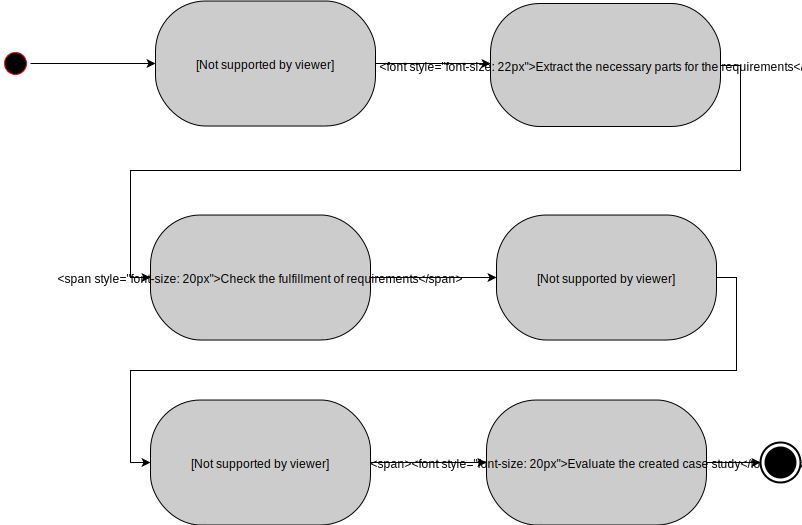
\includegraphics[scale=.45]{logos/Procedure.pdf}
\end{frame}

\subsection{Evaluation for CS}
\begin{frame}{Evaluation of the case study}


\includegraphics[scale=.55]{logos/OverviewEvalPresMethod.pdf}
\end{frame}

\section{Application to CoCoME}
\subsection{Step 1}
\begin{frame}{P1: Investigate the current state of CoCoME}
\includegraphics[scale=.5]{logos/Overview_CoCoME.pdf}\\
\end{frame}

\subsection{Step2_1}
\begin{frame}{P2: Requirements for privacy-considering case study}
\begin{table}
\centering
\begin{tabular}{|c|c|}
\hline 
\multicolumn{2}{|c|}{Requirements} \\ 
\hline 
R1 & Component-based system \\ 
\hline 
R2 & Definition of use cases \\ 
\hline 
R3 & Security relevant data \\ 
\hline 
R4 & Definition of user roles \\ 
\hline 
R5 & Definition of access rights \\ 
\hline 
R6 & Definition of the type of data processing in the components \\
\hline
\end{tabular} 
\end{table}
\end{frame}
\subsection{Step 2_1}
%TODO P2-P4
\begin{frame}{Procedure P2 -P4\\ Requirements R1-R4}
\begin{itemize}
\item \cmark : documented, \trimark : defined, \kmark : generated/ derived
\item R1: Component based system.  \cmark %Docu
\pause
\item R2: 13 use cases are defined in the documentation. \cmark % docu
\pause
\item R3: Security relevant data. \trimark% slebst erarbeitet
\begin{itemize}
\item Four different classes for the data in CoCoME.
\item The security relevance for each class was measured according to \cite{assetValue}.
\pause
\item Account data: security relevant 
\item Customer data: security relevant 
\item System data: security relevant
\item P\&S data: security relevant in composition with one of the other classes.
\end{itemize}
\pause
\item R4: 6 roles are defined in the documentation. \cmark | \trimark% doku + selbst 
\end{itemize}
\end{frame}

\subsection{ACM}
\begin{frame}{Procedure P2-P4\\ R5: access rights \kmark}
\begin{itemize}
\item Finer grained, high level form derived from (\cite{CaseStudyAndAccessrigths}).
\pause
\item Access control matrix (ACM)
\begin{itemize}
\item Level 1: \textbf{fullAccess}
\item Level 2: \textbf{AccessToUsedData}
\item Level 3: \textbf{AccessToOwnData}
\item Level 4: \textbf{default}
\end{itemize}
\end{itemize}
\begin{table}
\begin{tabular}{|c|c|c|}
\hline
Roles & Webfrontend & TS:Inventory \\
\hline
StockManager 
&
%WF
 \begin{tabular}{c|c}
Customer data & 4\\
Account data & 3\\
P\&S data & 2\\
System data & 4\\
\end{tabular}
&
%TS:inv
 \begin{tabular}{c|c}
Customer data & 4 \\
Account data & 3 \\
P\&S data & 2 \\
System data & 4 \\
\end{tabular}
  \\ 
\hline 
\end{tabular}
%\caption{Level 1: \textbf{fullAccess}, Level 2: \textbf{AccessToUsedData}, Level 3: \textbf{AccessToOwnData}, Level 4: \textbf{default}}
\end{table}
\end{frame}




\subsection{OpM}
\begin{frame}{Procedure P2-P4\\ R6: types of data processing in the system \kmark}
\begin{itemize}
\item We identified four categories of data processing in CoCoME.
\begin{itemize}
\item Transmission of data
\item alternation of data
\item relational algebra
\item I/O
\end{itemize}
\pause
\item Operations matrix(OpM)
\end{itemize}
\begin{tabular}{|c|c|c|c|c|}
\hline 
 Components & customer & account & P\&S & system \\ 
\hline 
Webfrontend & transmit & transmit & I/O, transmit & n/a \\ 
\hline 
\end{tabular} 
\end{frame}



\subsection{data flow}
\begin{frame}{Procedure P6: Definition of a scenario}
\begin{itemize}
\item Scenario: StockManager requests a report for the purchased products of a customer.
\end{itemize}
\begin{figure}
\begin{subfigure}{.4\textwidth}
\includegraphics[scale=0.35]{logos/PickUpShopPresentation.pdf}
\end{subfigure}%
\begin{subfigure}{.6\textwidth}
\includegraphics[scale=.25]{logos/DFUC13_Presentation.pdf}
\end{subfigure}
\end{figure}
\end{frame}

\section{Evaluation}
\subsection{gqmplan}
\begin{frame}{Goal-Question-Metric plan}
\includegraphics[scale=0.45]{logos/OverviewEvalPresShort.pdf}

\end{frame}
\subsection{evalCS}
\begin{frame}{Evaluation for the quality of the access rights}
\begin{itemize}
\item Evered and B\"ogeholz defined seven criteria to measure the quality of access rights.
\end{itemize}
\begin{table}
\centering
\begin{tabular}{|c|c|c|}
\hline 
\multicolumn{2}{|c|}{Access rights} & fulfilled \\ 
\hline 
Specification & Aspect-oriented & \cmark \\ 
\hline 
 & Positive & \cmark \\ 
\hline 
 & Need-to-know & \cmark \\ 
\hline 
Comprehensibility & Clear & ? \\ 
\hline 
 & Concise & ? \\ 
\hline 
Implementation & Fundamental & n/a \\ 
\hline 
 & Efficient & n/a \\ 
\hline 
\end{tabular} 

%\begin{tabular}{|c|c|}
%\hline 
%Access Rights & fulfilled? \\ 
%\hline 
%\multicolumn{2}{|c|}{Specification}\\
%\hline
%Aspect-oriented & \cmark \\ 
%\hline 
%Positive & \cmark \\ 
%\hline 
%Need-to-know & \cmark \\ 
%\hline 
%\multicolumn{2}{|c|}{Comprehension}\\
%\hline
%Concise & ? \\
%\hline
%Clear & ?\\
%\hline 
%\multicolumn{2}{|c|}{Realization}\\
%\hline
%Fundamental & n/a\\
%\hline 
%Efficient & n/a \\
%\hline
%\end{tabular} 
\end{table} 
\end{frame}

\subsection{Evaluation of covered information flow classes}
\begin{frame}{Evaluation of covered information flow classes}
\begin{itemize}
\item Problem statement: Non-influence = non-interference + non-leakage (\cite{Noninfluence}).
\begin{itemize}
\item Non-interference:  High data inputs in the program flow have no effect on low data outputs. 
\item Non-leakage: Unobservable if certain actions have taken place.
\end{itemize}
\end{itemize}


\pause
\begin{table}
\centering
\begin{tabular}{|c|c|} 
\hline 
Data flow & fulfilled? \\ 
\hline 
Illegal information flow & \cmark \\ 
\hline 
Information flow from high to low & \cmark \\  
\hline 
Direct information flow between roles & \xmark \\ 
\hline 
No observable information  flow & \xmark \\
\hline 
\end{tabular}
\end{table}
\end{frame}

\subsection{TtoV}
\begin{frame}{Threats to validity}
\begin{table}
\centering
\begin{tabular}{|c|c|c|c|}
\hline 
Internal & External & Construct & Conclusion \\ 
Validity & Validity & Validity & Validity\\
\hline 
II, III & I & II & III \\ 
\hline 
\end{tabular} 
\end{table}
\begin{itemize}
\item I:   Not  applied to various systems.
\item II:  Not all access rights criteria were checked. 
\item III: Not all information flow classes are covered.
\end{itemize}
\end{frame}



\section{Conclusion}
\subsection{Future work}
\begin{frame}{Future work}
\begin{itemize}
\item Evaluation of the procedure:
\begin{itemize}
\item Create a case study for the complete CoCoME system.
\item Apply the procedure to other systems (e.g Travelsystem (\cite{Travelsystem})) and create further case studies.
\end{itemize}
\item Case study
\begin{itemize}
\item Short term work
\begin{itemize}
\item Evaluate the criteria \textit{concise} and \textit{clear}. 
\item Define additional scenarios to cover all information flow classes.
\end{itemize}

\item Long term work
\begin{itemize}
\item Evaluate the criteria \textit{fundamental} and \textit{efficient}.
\item Definition of further information flow classes other than non-influence. 
\item Using the case study for evaluating a data based privacy analysis.
\end{itemize}
\end{itemize}

\end{itemize}
\end{frame}


\subsection{PIBA}
\begin{frame}{PIBA}
\begin{itemize}
\item Problem
\begin{itemize}
\item Usable case studies for evaluating data-based privacy analysis (DBPA) are difficult to create.
\end{itemize}
\item Idea
\begin{itemize}
\item Introduce a method for creating usable case studies for DBPA approaches.
\end{itemize}
\item Benefit
\begin{itemize}
\item Comparability for different privacy analysis approaches.
\end{itemize}
\item Actions
\begin{itemize}
\item Create a method for the creation of case studies.
\item Apply the method to a system.
\item Evaluate the created case study.
\end{itemize}
\end{itemize}
\end{frame}



\appendix
\beginbackup


\begin{frame}[allowframebreaks]{References}
\printbibliography
\end{frame}

\begin{frame}{Evaluation Modeling language}
\begin{table}
\begin{tabular}{|c|c|}
\hline 
Meta model  & possible ? \\ 
\hline 
relational algebra & yes \\ 
\hline 
I/O operations & yes \\ 
\hline 
Transmission of data & yes \\ 
\hline 
Change of access rights & yes \\ 
\hline 
Alternation of data & yes \\ 
\hline 
ACM in system model & no \\
\hline
\end{tabular} 
\end{table}
\end{frame}

\begin{frame}{Operations matrix complete}
\begin{table}
\begin{tabular}{|c|c|c|c|c|}
\hline 
Types of  & customer & account & P\& S & system  \\ 
data processing  & & & & \\
\hline 
Webfrontend &  transmit & transmit & I/O & n/a \\ 
& & &  transmit & \\
\hline 
PickupShop &  transmit & transmit & I/O, & n/a \\ 
& & & transmit & \\
\hline 
Tradingsystem:& change & change & change & n/a \\ 
inventory:app & transmit& transmit & & \\
\hline 
Tradingsystem: & rel. algebra& rel. algebra& rel. algebra& change \\
inventory:data & operations & operations & operations & \\ 
\hline
Tradingssystem: & change & non-existent & change & n/a \\
cashdeskline & transmit &  & transmit & \\
\hline 
\end{tabular} 

\end{table}
\end{frame}

\begin{frame}{Definition of the value of an asset}
\begin{itemize}
\item Different assets in system are related to each other.
\item The assets are categorized in different levels. The value of an asset to the system is decreasing with descending numbers.
\item A higher level is more crucial to protect for the system than the lower levels.
\item In CoCoME:
\begin{itemize}
\item Level 1: Customer and account data 
\item Level 2: System and P\& S data
\end{itemize}
\end{itemize}
\end{frame}

\begin{frame}{Conclusion of the Procedure}
\begin{itemize}
\item In the current state, we would argue it depends on the use of the resulting case study.
\item Conclusion of the procedure
\begin{itemize}
\item Access rights:
\begin{itemize}
\item Concluded, further fulfillment of the criteria were not possible due to time constraints.
\end{itemize}
\item Information flow classes
\begin{itemize}
\item If the covered information flow classes are sufficient for the intended use use of the case study
\end{itemize}
\end{itemize}
\item No Conclusion of the procedure
\begin{itemize}
\item Information flow classes are not covered yet.
\end{itemize}
\end{itemize}
\end{frame}

\backupend

\end{document}
